\documentclass[tikz,border=2pt,11pt]{standalone}
\usetikzlibrary{arrows.meta}
\usetikzlibrary{positioning}
\usepackage{amsmath}
\usepackage{amssymb}
\usepackage{tikz}
\newcommand{\R}{\mathbb R}
\newcommand{\N}{\mathbb N}
\newcommand{\E}{\mathbb E}
\newcommand{\Prob}{\mathbb P}
\newcommand{\sphere}{S^{d-1}}
\newcommand{\norm}[1]{\left\lVert #1\right\rVert}
\newcommand{\ip}[2]{\langle #1,#2\rangle}
\newcommand{\ind}{\mathbf 1}
\newcommand{\dist}{\operatorname{dist}}
\newcommand{\supp}{\operatorname{supp}}
\newcommand{\aff}{\operatorname{aff}}
\newcommand{\vol}{\operatorname{vol}}
\newcommand{\op}{\mathrm{op}}
\DeclareMathOperator{\rank}{rank}
\begin{document}
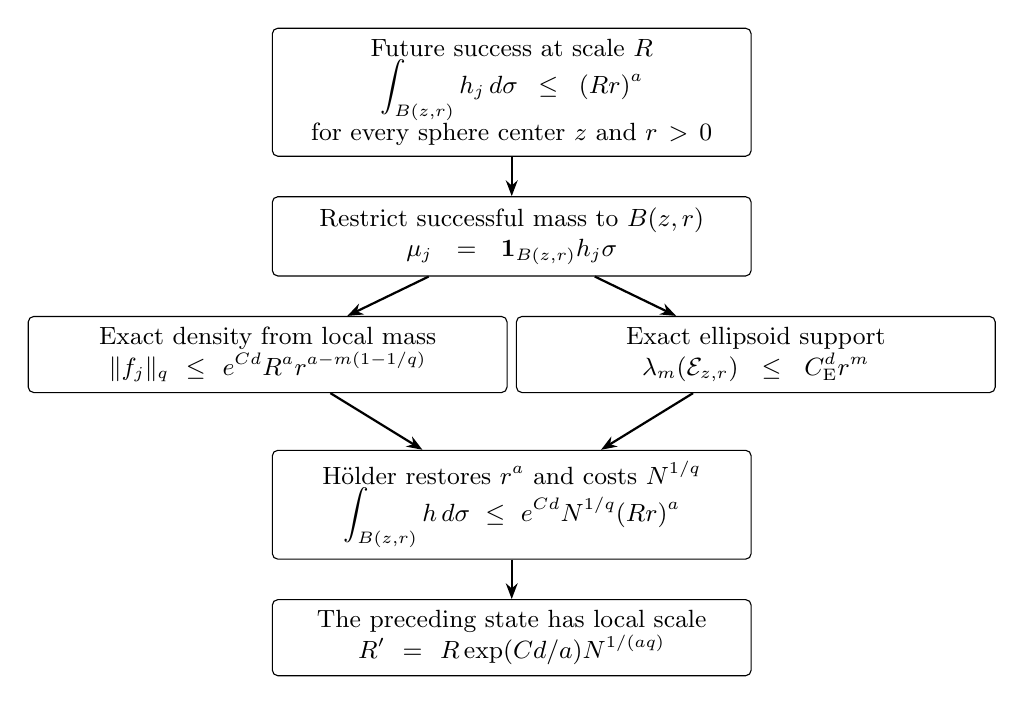
\begin{tikzpicture}[
 box/.style={draw,rounded corners=2pt,align=center,text width=5.8cm,
             inner sep=4pt,font=\small},
 arrow/.style={-{Stealth[length=2mm]},thick},node distance=5mm and 4mm]
\node[box] (local) {Future success at scale \(R\)\\
 \(\displaystyle\int_{B(z,r)}h_j\,d\sigma\le(Rr)^a\)\\
 for every sphere center \(z\) and \(r>0\)};
\node[box,below=of local] (measure) {Restrict successful mass to \(B(z,r)\)\\
 \(\mu_j=\mathbf1_{B(z,r)}h_j\sigma\)};
\node[box,below=of measure,xshift=-3.1cm] (moment) {Exact density from local mass\\
 \(\|f_j\|_q\le e^{Cd}R^a r^{a-m(1-1/q)}\)};
\node[box,below=of measure,xshift=3.1cm] (support) {Exact ellipsoid support\\
 \(\lambda_m(\mathcal E_{z,r})\le C_{\mathrm E}^d r^m\)};
\node[box,below=22mm of measure] (holder) {H\"older restores \(r^a\) and costs \(N^{1/q}\)\\
 \(\displaystyle\int_{B(z,r)}h\,d\sigma\le e^{Cd}N^{1/q}(Rr)^a\)};
\node[box,below=of holder] (output) {The preceding state has local scale\\
 \(R'=R\exp(Cd/a)N^{1/(aq)}\)};
\draw[arrow] (local)--(measure);
\draw[arrow] (measure)--(moment);
\draw[arrow] (measure)--(support);
\draw[arrow] (moment)--(holder);
\draw[arrow] (support)--(holder);
\draw[arrow] (holder)--(output);
\end{tikzpicture}
\end{document}
